\section{Prefix sum}
\label{sec:prefix_sum}


The all-prefix-sums operation (also referred to as prefix sum or simply scan) is a simple calculation which is most often found as part of larger and more complex routines. It serves as fundamental building block for implementing well-known algorithms such as radix sort (covered in chapter \ref{sec:sorting_radix}), stream compacting, minimum spanning tree and many more (cf. Blelloch's papers on prefix sum \cite{scan_blelloch_examples} \cite{scan_blelloch} and the GPU Gems 3 chapter 39.1 \cite{gpu_gems_3_chapter_39}).

The all-prefix-sums operation uses a binary associative operator $\oplus$ with identity element $I$ to transforms an input array of $n$ elements

\begin{equation*}
[a_0, a_1, \dots, a_{n-1}]
\end{equation*}

into an output array of $n$ elements where

a) each output element is the sum of all elements preceding the corresponding input element. This is known as an exclusive scan. \cite{gpu_gems_3_chapter_39}

\begin{equation*}
[I, a_0, (a_0 \oplus a_1), \dots, (a_0 \oplus a_1 \oplus \dots \oplus a_{n-2})]
\end{equation*}

b) each  output element is the sum of all elements preceding the corresponding input element and the input element itself. This is known as an inclusive scan. \cite{gpu_gems_3_chapter_39}

\begin{equation*}
[a_0, (a_0 \oplus a_1), \dots, (a_0 \oplus a_1 \oplus \dots \oplus a_{n-1})]
\end{equation*}

Contrary to the matrix multiplication of the previous chapter \ref{sec:matrix_mul} the all-prefix-sums operation does not offer similarly trivial parallelism. Scanning an array is naturally sequential with a complexity of $\mathcal{O}(n)$. Although each output element could be calculated independently to gain parallelism, a lot of redundant work would be necessary raising the overall complexity to $\mathcal{O}(n^2)$ with the last element still taking $\mathcal{O}(n)$ time to calculate.
The following chapter will focus on efficient and parallel implementations of an exclusive scan (except otherwise noted) using addition as operator on an input array of integers. This chapter is orientated towards the excellent Parallel Prefix Sum article from GPU Gems 3 \cite{gpu_gems_3_chapter_39}.


\subsection{CPU Implementation}

Implementing a sequential, single threaded scan for the CPU is simple. The first output element is initialized to zero. We than loop over the remaining output elements and set each one to the value of its predecessor plus the corresponding input element. Listing \ref{lst:scan_cpu} shows an example of a scan implementation.

\lstset{basicstyle=\ttfamily{}\scriptsize{}}
\lstinputlisting[language=C++, caption=A simple C++ implementation of an exclusive scan for the CPU., label=lst:scan_cpu, firstline=34, lastline=39]{code/scan/main.cpp}
\lstset{basicstyle=\ttfamily{}}

This code performs exactly $n - 1$ additions which is the minimum number of additions required to produce an exclusive scan of an array with $n$ elements. Concerning the following parallel scan implementations later in this chapter we would like them to be work-efficient. This means that the parallel implementation should have the same work complexity of $\mathcal{O}(n)$ as the sequential one.

\begin{quote}
A parallel computation is work-efficient if it does asymptotically no more work (add operations, in this case) than the sequential version \cite{gpu_gems_3_chapter_39}.
\end{quote}

The benchmark of this algorithm in figure \ref{fig:scan_chart} confirms the linearity of scan. Furthermore we can also see that scanning is a quite fast operation (when e.g. being compared to the matrix multiplication of the previous chapter \ref{sec:matrix_mul}). The CPU implementation manages to scan $2^{26}$ elements (256 MiB of data) in 215 ms.

\subsection{Naive GPU implementation}

The first GPU implementation is base on the article Data Parallel Algorithms written by Hillis and Steele in 1986 \cite{scan_naive}. Their approach to compute an inclusive (!) scan is shown in figure \ref{fig:scan_naive}. The algorithm uses several passes to compute the final output array in place. In each pass the value of a predecessor is added to an element. The offset from each element to its predecessor is determined by the pass index and is $2^{d - 1}$ where d is the number of the pass starting with 1.

\begin{figure}
\centering
\includegraphics[width=0.5\linewidth]{scan_naive}
\caption{A naive approach for a parallel scan \cite{scan_naive}. (figure from GPU Gems 3 \cite{gpu_gems_3_chapter_39})}
\label{fig:scan_naive}
\end{figure}

By now the algorithm assumes that in each pass all input elements are read before any output elements are written. This can only be achieved if this algorithm is run on a device with as many cores as input elements to ensure correct read and write ordering. This is usually not the case for larger arrays (current GPUs have around a few thousands cores. cf. NVIDIA Kepler GK110 in chapter \ref{sec:gpu}). A solution to this problem is double buffering. Instead of computing the partial sums in place inside the input array, a second equally sized buffer is created. In each pass input data is read from one of the buffers and written to the other. Before the next pass the buffers are swapped.
Listing \ref{lst:scan_naive_host} shows an example host code implementing this approach.

\lstset{basicstyle=\ttfamily{}\scriptsize{}}
\lstinputlisting[language=C++, caption=Host code for the naive scan algorithm., label=lst:scan_naive_host, firstline=41, lastline=71]{code/scan/main.cpp}
\lstset{basicstyle=\ttfamily{}}

At first, two buffers with the size of the input are created. Both of them have to be read- and writable as they are read from and written to alternatingly when executing the passes. The source buffer is filled with the input data. Although this algorithm is independent from the chosen work group size, we have to round the number of enqueued work items (one for each input element) up to be a multiple of the work group size. This \lstinline!adjustedWorkSize! will be the size of the enqueued ND range. After this short setup the passes are executed. Each pass corresponds to a power of two (loop variable \lstinline!offset!, cf. figure \ref{fig:scan_naive}) which corresponds to the offset of an element to the predecessor that should be added to it. This offset is raised each pass until it is larger than the problem size. The kernel is executed once for each pass, given the source and destination buffer, the offset and the original problem size as arguments. At the end of a pass the source and destination buffers are swapped (only the handles, not the actual contents). After the last pass has been executed, the result is read from the source buffer (the last pass wrote to the destination buffer which was swapped with the source buffer at the end of the loop).
Listing \ref{lst:scan_naive_kernel} shows the kernel code corresponding to the host code from listing \ref{lst:scan_naive_host}.

\lstset{basicstyle=\ttfamily{}\scriptsize{}}
\lstinputlisting[language=CL, caption=OpenCL Kernel code for the naive scan algorithm., label=lst:scan_naive_kernel]{../src/scan/gpu/thesis/NaiveScan.cl}
\lstset{basicstyle=\ttfamily{}}

The kernel starts by querying the id of the current element. If this id is larger than the actual problem size, the kernel returns. This case can happen when the problem size has been rounded up to be a multiple of the chosen work group size. If the id addresses a valid input element, we determine if this element has a predecessor at the current pass' offset. If this is the case, the input element is read from the source buffer, added to its predecessor (also read from the source buffer) and written to the destination buffer. If the predecessor offset is to large, the input element remains the same, but has to be copied if it was just calculated in the last pass to keep the buffers consistent.

When we have a look at the benchmark of this algorithm and compare the results with the CPU implementation we can clearly see, that this approach does not profit very well from the large computational power GPUs offer. With 1148 milliseconds at $2^{26}$ elements the naive GPU version is five times slower than the CPU version. The low performance has basically two reasons. The first is the high number of kernel invocations necessary to compute the final result. For $21{26}$ input elements to scan, 26 passes are necessary each consisting of $2^{26}$ work items performing one addition leading to a runtime/work complexity of $\mathcal{O}(n log n)$. Compared with the complexity of the original CPU implementation which was $\mathcal{O}(n)$ this algorithm is not work-efficient. The second flaw of this implementation is the high rate of global memory access. Both buffers are accessed multiple times at the same locations throughout the passes. As the scan operation using a simple addition is more memory bound than computational, a lot of time is wasted on waiting for global memory transactions.
Fortunately, both problems can be tackled which will be subject to the following chapters.


\subsection{Work efficient GPU implementation}

tree based approach (GPU Gems) work efficiency?

\begin{figure}
\centering
\includegraphics[width=0.5\linewidth]{scan_work_efficient_up_sweep}
\caption{The up-sweep phase of a work efficient parallel scan \cite{scan_blelloch}.  (figure from GPU Gems 3 \cite{gpu_gems_3_chapter_39})}
\label{fig:scan_work_efficient_up_sweep}
\end{figure}

\begin{figure}
\centering
\includegraphics[width=0.5\linewidth]{scan_work_efficient_down_sweep}
\caption{The down-sweep phase of a work efficient parallel scan \cite{scan_blelloch}.  (figure from GPU Gems 3 \cite{gpu_gems_3_chapter_39})}
\label{fig:scan_work_efficient_down_sweep}
\end{figure}

\lstset{basicstyle=\ttfamily{}\scriptsize{}}
\lstinputlisting[language=C++, caption=Host code for the efficient scan algorithm., label=lst:scan_work_efficient_host, firstline=73, lastline=120]{code/scan/main.cpp}
\lstset{basicstyle=\ttfamily{}}

\lstset{basicstyle=\ttfamily{}\scriptsize{}}
\lstinputlisting[language=CL, caption=OpenCL Kernel code for the work efficient scan algorithm., label=lst:scan_work_efficient_kernel]{../src/scan/gpu/thesis/WorkEfficientScan.cl}
\lstset{basicstyle=\ttfamily{}}

\subsection{Recursively scanning blocks in local memory}

\begin{figure}
\centering
\includegraphics[width=0.5\linewidth]{scan_recursive}
\caption{Scanning larger arrays of values recursively \cite{gpu_gems_3_chapter_39}.}
\label{fig:scan_recursive}
\end{figure}

\lstset{basicstyle=\ttfamily{}\scriptsize{}}
\lstinputlisting[language=C++, caption=Host code for the recursive scan algorithm., label=lst:scan_recursive_host, firstline=123, lastline=170]{code/scan/main.cpp}
\lstset{basicstyle=\ttfamily{}}

\lstset{basicstyle=\ttfamily{}\scriptsize{}}
\lstinputlisting[language=CL, caption=OpenCL Kernel code for the recursive scan algorithm., label=lst:scan_recursive_kernel, firstline=1, lastline=65]{../src/scan/gpu/thesis/RecursiveScan.cl}
\lstset{basicstyle=\ttfamily{}}

\subsection{Optimization using vector types}

\lstset{basicstyle=\ttfamily{}\scriptsize{}}
\lstinputlisting[language=C++, caption=Host code for the recursive scan algorithm using vector types., label=lst:scan_recursive_vector_host, firstline=123, lastline=170]{code/scan/main.cpp}
\lstset{basicstyle=\ttfamily{}}

\lstset{basicstyle=\ttfamily{}\scriptsize{}}
\lstinputlisting[language=CL, caption=OpenCL Kernel code for the recursive scan algorithm using vector types., label=lst:scan_recursive_vector_kernel, firstline=1, lastline=149]{../src/scan/gpu/thesis/RecursiveScan.cl}
\lstset{basicstyle=\ttfamily{}}

\begin{figure}
\centering
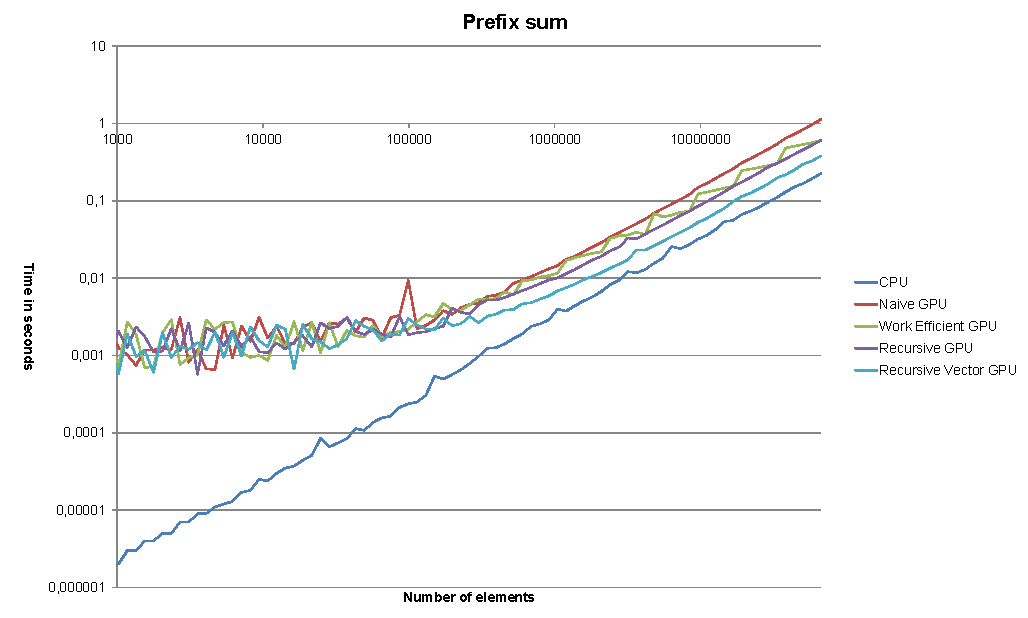
\includegraphics[width=\linewidth]{scan_chart}
\caption{Benchmark of several prefix sum implementations. The chart is based on the benchmark data in appendix chapter \ref{sec:scan_chart_data}. Note that both axis are of logarithmic scale.}
\label{fig:scan_chart}
\end{figure}

\subsection{Existing implementations}
Apple
libCL
(AMD APP SDK Samples)
NVIDIA OpenCL Samples
common diagram

\subsection{Conclusion}
Why linear problems are still required on GPUs? (as building block for other algorithms)
common diagram
